\scanpage{587}
\mspage{597}
\[
(51)\qquad
\left\{\begin{aligned}
a&=\varepsilon_3(\tau')\alpha^{-1}u
&\text{i.e.}\quad \alpha&=ua^{-1}\varepsilon_3(\tau')\\
b&=\beta^{-1}u
&\text{i.e.}\quad \beta&=ub^{-1}
\end{aligned}\right.\ ,
\]
I wonder whether this set-theoretic section of
$S_0\Gamma_{\rho,\sigma}^{!}$ over
$Z_{\rho,\sigma}^{!}=M^{!}[0]$ is multiplicative,
\unsure{or}, which amounts to the same thing,
whether $a$ and $b$ defined by (51) depend multiplicatively on
\deleted{\unsure{these}} $u$.

\uline{Proposition}. Let $(u,a,b)\in S_0\Gamma_{\rho,\sigma}^{!}$
(cf. (50)). For us to have $i=0$, $\unsure{j=0}$, i.e. for us to
have (51) --- i.e. for $(u,a,b)$ \deleted{\unsure{to be}}
to belong to the preceding set-theoretic section --- it is necessary and sufficient
that we have the relations
\[
(52)\qquad u\equiv b\equiv\varepsilon_3(\sigma)a\,
\deleted{\unsure{(\widehat\Pi_0)}}\quad\bmod\widehat\Pi_0.
\]
\margin{\figure{\begin{tikzpicture}
\draw (0,0)--(0,-2.6);
\end{tikzpicture}}}
\margin{where we have put
$\displaystyle\varepsilon_3(\sigma)=
\left\{\begin{array}{ll}1&\text{if }\varepsilon_3=+1\\
\sigma&\text{if }\varepsilon_3=-1\end{array}\right.$}

\margin{\uline{N.B.}\quad $\tau'\tau=\sigma^{-1}$\quad
$\tau'\sigma^{-1}=\tau$.}

\uline{Proof}. Since
$\beta\deleted{\unsure{\in}}\inserted{=ub^{-1}}$ and
\deleted{$\unsure{\alpha\varepsilon_3(\tau')=ua^{-1}}$}
\inserted{$\deleted{\unsure{\alpha}}\alpha\varepsilon_3(\tau)
=\deleted{\unsure{ua}}ua^{-1}\varepsilon_3(\tau'\tau)
=ua^{-1}\varepsilon_3(\sigma^{-1})$}
are both in $\unsure{\widehat\Pi_0}$, the condition is
necessary. For sufficiency, we note that (52) reads, with the
notation of (50),
\inserted{\unsure{where} $f=ub^{-1}$, $f'=ua^{-1}$ i.e.
$f'\varepsilon_3(\sigma^{-1})=ua^{-1}\varepsilon_3(\sigma^{-1})$
\deleted{\unsure{i.e.} $f'\varepsilon_3(\unsure{\sigma})$}}
\deleted{$f,\unsure{f'}\in\Pi_0$},
\inserted{\[
\deleted{\unsure{f\in\Pi_0}}\qquad
(53)\quad f,f'\varepsilon_3(\sigma^{-1})\in\Pi_0
\]
\deleted{\unsure{1}}}
and reducing modulo $\Pi_0$ in $\unsure{\widehat G}/\Pi_0$
this reads $\unsure{\dot\beta}\dot\sigma^{i}=1$ and
\deleted{$\unsure{\dot\alpha\dot\rho^{j}\varepsilon_3(\dot\tau)=1}$ i.e.},
\inserted{$\dot\alpha\dot\rho^{j}\varepsilon_3(\tau'\sigma^{-1})^{\cdot}=1$,
this last relation also reads
$\dot\alpha\dot\rho^{j}\varepsilon_3(\tau)^{\cdot}=1$ i.e.}
\deleted{this last relation also reads}
$\unsure{\varepsilon_3(\dot\tau)\dot\alpha\dot\rho^{j}=1}$,
\deleted{so the relation becomes}
$\varepsilon_3(\dot\tau)\dot\alpha\dot\rho^{j}=1$
now $\varepsilon_3(\dot\tau)\dot\alpha\unsure{=}1$,
the condition is
\deleted{$\varepsilon_3(\dot\tau)\dot\alpha=1$ so the relation}
\[
\deleted{\unsure{(53)}}\qquad
\dot\sigma^{i}=\dot\rho^{j}=1\qquad\text{i.e.}\quad i=0,\ j=0
\]
\unsure{q.e.d.}.

\deleted{\uline{Corollary}\quad The section under consideration is multiplicative.}
\mspage{586}

\scanpage{588}
\deleted{At the same time, this suggests to us a modification of the constructions
of the preceding sections, replacing the fiber products over
$\unsure{\gamma_{\rho,\sigma}}=
\deleted{\unsure{\Gamma_{\rho,\sigma}\rtimes}}
G_{\rho,\sigma}/\unsure{G}_{\rho,\sigma}^{+}$
by fiber products over \deleted{$\unsure{\Gamma_{\rho}}$}
the finer group $G_{\rho,\sigma}/\Pi_0$, which
\deleted{\unsure{is a}}\inserted{\unsure{of which}} the
universal \unsure{covering|group} is a covering of degree 12 of this one.}

\unsure{Let|Let} now $u$, corresponding to $a,b,\varepsilon_3$
and $u'$, corresponding to $a',b',\varepsilon_3'$, let
$u''=u'u$, corresponding to $a''$, $b''=b'b$ and
$\varepsilon_3''=\varepsilon_3'\varepsilon_3$, so that we shall have
\[
\begin{array}{rcll}
u&\equiv&\varepsilon_3(\sigma)a&(\widehat\Pi_0)\\
u'&\equiv&\varepsilon_3'(\sigma)a'&(\unsure{\widehat\Pi_0})\\
u''&\equiv&\underbrace{\varepsilon_3''(\sigma)}a''&(\widehat\Pi_0)\\
\Vert&&&\\[-1ex]
u'u&\equiv&\deleted{\unsure{\varepsilon_3''(\sigma)}}
\varepsilon.\varepsilon_3'(\sigma).\varepsilon_3(\sigma).a''&
\begin{gathered}\text{where }\varepsilon\in\{\pm1\},\ \varepsilon=-1\text{ iff}\\
\varepsilon_3=-1\quad\text{\uuline{and}}\quad\varepsilon_3'=-1
\end{gathered}\\
\vert\!\vert\!\vert&&&\\[-1ex]
(\varepsilon_3'(\sigma)a')(\varepsilon_3(\sigma)a)&&&
\end{array}
\]
\margin{$\unsure{=}$}
\margin{\unsure{!}}

which gives
\[
a'\varepsilon_3(\sigma)a\equiv\varepsilon\varepsilon_3(\sigma)a''
\quad(\widehat\Pi_0)\qquad\text{i.e.}
\]
\[
(53)\qquad a''\equiv\varepsilon\varepsilon_3(\unsure{\sigma|\sigma^{-1}})(a').a
\]
\margin{N.B. $\varepsilon_3(\sigma)$ and $\varepsilon_3(\sigma^{-1})$
operate in the same way.}

Thus the expected relation
\[
a''=a'a\qquad\text{equivalent to}\quad a''\equiv a'a\quad(\widehat\Pi_0)
\]
is true if and \uline{only if}
\inserted{\deleted{\deleted{$\unsure{a''=\varepsilon}$}
(where $\varepsilon\in\{\pm1\}$ and $\varepsilon=-1$ iff
$\varepsilon_3=\varepsilon_3'=-1$}}
\deleted{\[
(54)\qquad\varepsilon_3(\sigma)(a')\equiv\varepsilon a'
\quad(\widehat\Pi_0)
\deleted{\unsure{(\widehat\Pi_0\tau)}}
\deleted{\unsure{\varepsilon_3(a')=\varepsilon a'}}.
\]}
\deleted{which \unsure{for} $\varepsilon_3$}
\deleted{\unsure{condition which}}
\deleted{This condition breaks down according to \unsure{the|these} cases:
$\unsure{\tau'},a'$ are the images of $\unsure{\tau'},a'$ in
$\unsure{M}/\widehat\Pi_0$.}
\deleted{\inserted{This condition is automatically satisfied}}

\margin{\diagram{\begin{tikzcd}[ampersand replacement=\&,row sep=small,column sep=large]
\deleted{\boxed{54\text{bis}}} \& \\
\deleted{1)\ \varepsilon_3=\varepsilon_3'=1:\ \text{always OK}} \& \\
\deleted{2)\ \varepsilon_3=1,\ \varepsilon_3'=-1:\ \text{always OK}} \& \\
\deleted{3)\ \varepsilon_3=-1,\ \varepsilon_3'=1:\
\boxed{\sigma(a')\equiv a'\ (\widehat\Pi_0)}}
\arrow[r,"\deleted{\text{i.e.}}"] \&
\deleted{\boxed{\sigma(u')\equiv u'\ (\widehat\Pi_0)}}\\
\deleted{4)\ \varepsilon_3=-1,\ \varepsilon_3'=-1:\
\boxed{\sigma(a')\equiv-a'\ (\widehat\Pi_0)}}
\arrow[r,"\deleted{\text{i.e.}}"] \&
\deleted{\boxed{\sigma(u')\equiv-u'\ (\widehat\Pi_0)}}
\end{tikzcd}}}
\mspage{587}

\scanpage{589}
\mspage{598}
\[
(54)\qquad\varepsilon_3(\sigma)(a')\equiv\varepsilon a'
\quad(\unsure{\Pi_0|\widehat\Pi_0}),\quad
\text{where }\left\{\begin{array}{l}
\varepsilon\in\{\pm1\},\quad
\varepsilon\overset{\unsure{\mathrm{dfn}}}{=}-1
\text{ iff }\varepsilon_3=\varepsilon_3'=-1\\
\varepsilon_3(\sigma)\overset{\unsure{\mathrm{dfn}}}{=}
\left\{\begin{array}{ll}1&\text{if }\varepsilon_3=+1\\
\sigma&\text{if }\varepsilon_3=-1\end{array}\right.
\end{array}\right.
\]
This condition (54) can be spelled out according to the cases:
\[
(55)\quad\left\{\begin{array}{ll}
a)&\text{if }\varepsilon_3=1,\ \text{then }\varepsilon=1
\text{ and (54) always satisfied}\\
b)&\text{if }\varepsilon_3=-1,\ \text{then (54) reads}\quad
\deleted{\unsure{\varepsilon_3}}\ \sigma(a')\equiv\varepsilon_3'.a'
\quad(\widehat\Pi_0)\quad\text{i.e.}\\
&[\dot\sigma,\dot a']=\dot\varepsilon_3'
\end{array}\right.
\]
\margin{where the $\cdot$ denote the classes in $M/\widehat\Pi_0$}

Since we have
\[
a'\equiv\varepsilon_3'(\sigma)^{-1}u'
=\left\{\begin{array}{ll}
u'&\text{if }\varepsilon_3'=1\\
\sigma^{-1}u'&\text{if }\varepsilon_3'=-1
\end{array}\right.\ ,
\]
we find that condition (55, b) is also equivalent to:
\[
(56)\quad\deleted{\unsure{[\dot\sigma,\dot u']=\varepsilon_3'}}
\left\{\begin{aligned}
\dot\sigma(\dot u')&=\unsure{\dot\varepsilon_3'|\varepsilon_3'}\dot u'
\quad\text{in }M/\widehat\Pi_0,\quad\text{i.e.}\\
[\dot\sigma,\dot u']&=\unsure{\dot\varepsilon_3'|\varepsilon_3'}
\end{aligned}\right.
\]
(\inserted{\uline{equivalence}} Valid both for
$\varepsilon_3'=1$ and $\varepsilon_3'=-1$).

Now we have seen (35) that we have in $\unsure{\widehat G/\widehat\Pi_0}$)
\[
\dot u'(\dot\sigma)=\varepsilon_2(u')\dot\sigma
\]
i.e.
\[
[\dot u',\dot\sigma]=\varepsilon_2(u')\quad\text{or again}
\]
\[
(57)\qquad[\dot\sigma,\dot u']=\varepsilon_2(\unsure{\dot u'|\widehat u'})^{\cdot}.
\]
Comparing (56) and (57), we see that (56) takes the equivalent form
\[
(58)\qquad\varepsilon_2(u')=\varepsilon_3(u').
\]
We have thus proved:

\uline{Proposition}. Let $u,u'$, and $u''=u'u\in M^{!}[0]=Z_{\rho,\sigma}^{!}$,
corresponding to
$\varepsilon_3\unsure{,|\ne}\varepsilon_3',\
\varepsilon_3''=\varepsilon_3'\varepsilon_3\in\{\pm1\}$, and:
\[
a=\varepsilon_3(\tau')\alpha^{-1}u,\quad
a'=\varepsilon_3'(\tau')\alpha'^{-1}u',\quad
a''=\underbrace{\varepsilon_3''(\tau')}_{\inserted{\varepsilon_3'(\tau')\varepsilon_3(\tau')}}
\alpha''^{-1}\underbrace{u''}_{\inserted{u'u}},
\]
\inserted{with $a,a',a''\in\unsure{N_\rho'|N_\rho^{*}}$,
$a\equiv\varepsilon_3(\sigma)^{-1}u$, $a'\equiv\ldots$, $a''\equiv\ldots$
$(\Pi_0)$}
\deleted{In order that} The following conditions are equivalent:

\margin{\uline{N.B.}\quad
$\displaystyle\left\{\begin{aligned}
\varepsilon_3&=\varepsilon_3(u)=\varepsilon_3(a)\\
\varepsilon_3'&=\varepsilon_3(u')=\varepsilon_3(a')\\
\varepsilon_3''&=\varepsilon_3(u'')=\varepsilon_3(\unsure{a''|a'})
\end{aligned}\right.$}
\mspage{588}

\scanpage{590}
\[
\begin{array}{ll}
a)\ \text{We have}&a''=a'a\\[1ex]
\unsure{a')}\ \text{We have}&a''\equiv a'a\quad(\widehat\Pi_0)\\[1ex]
\unsure{b)}\ \text{We have}&
\varepsilon_3\deleted{\unsure{a}}=1\,
\inserted{\text{i.e. }a(\rho)=\rho}\quad\text{\uline{or}}\quad
\sigma(a')\equiv\varepsilon_3'a'\quad(\widehat\Pi_0)\\[1ex]
b')\ \text{We have}&
\varepsilon_3=1\,
\inserted{\text{i.e. }a(\rho)=\rho}\quad\text{\uline{or}}\quad
\unsure{\dot a'|a'}(\sigma)\equiv\varepsilon_3'\sigma
\quad(\unsure{\widehat\Pi_0|\overline\Pi_0})\\[1ex]
c)\ \text{We have}&
\varepsilon_3=1\,
\inserted{\text{i.e. }a(\rho)=\rho}\quad\text{\uline{or}}\quad
\deleted{\unsure{\varepsilon_3=1}}\ \sigma(\unsure{u'})\equiv
\varepsilon_3'u'\quad(\widehat\Pi_0)\\[1ex]
c')\ \text{We have}&
\varepsilon_3=1\ \inserted{\text{i.e. }a(\rho)=\rho},
\quad\text{\uline{or}}\quad
\unsure{u'|\dot u'}(\sigma)\equiv\varepsilon_3'\sigma
\quad(\widehat\Pi_0)\\[1ex]
d)\ \text{We have}&
\boxed{\begin{array}{l|l}
\varepsilon_3=1\quad\text{or}\quad\varepsilon_2'=\varepsilon_3'\quad\text{i.e.}
&\varepsilon_2'\varepsilon_3'=1
\end{array}}
\end{array}
\]

\uline{Corollary}\quad Over the two subgroups
\[
(59)\quad\left\{\begin{aligned}
\unsure{Z_{\rho,\sigma}^{!'}}&=\unsure{M^{!'}}[0]
\overset{\unsure{\mathrm{dfn}}}{=}
\{u\in Z_{\rho,\sigma}^{!}\mid\varepsilon_3(u)=1\}\\
Z_{\rho,\sigma}^{!'''}&=M^{!'''}[0]
\overset{\unsure{\mathrm{dfn}}}{=}
\{u\in Z_{\rho,\sigma}^{!}\mid\varepsilon_2(u)=\varepsilon_3(u)\}
\end{aligned}\right.
\]
the set-theoretic section map

$(60)\quad A:$
\diagram{\begin{tikzcd}[ampersand replacement=\&,row sep=small,column sep=large]
Z_{\rho,\sigma}^{!}\arrow[r]\arrow[d,equal]
\& S_0\Gamma_{\rho,\sigma}^{!}\\
M^{!}[0]\&\unsure{\ni}\\
\unsure{\cdot}u\arrow[r,mapsto]
\& (u,\ a=\varepsilon_3(\tau')\alpha^{-1}u,\ b=\beta^{-1}u)
\end{tikzcd}}
\margin{cf. proposition page 597}

is a multiplicative section. But it is not multiplicative
over $\unsure{M^{!}}[0]$ as a whole.
\mspage{589}

\scanpage{591}
\mspage{599}
\uline{Remark}\quad The elements of the inverse \unsure{image|image}
$S_0\Gamma_{\rho,\sigma}^{\unsure{'!|!'}}$ of $Z_{\rho,\sigma}^{!'}$
in $S_0\Gamma_{\rho,\sigma}^{!}$ which belong to the section under consideration
are characterized (by virtue of the proposition on page 598) by the relation
\[
(61)\qquad u\equiv b\equiv a\quad\bmod\widehat\Pi_0
\]
\margin{(in addition to $\varepsilon_3(u)=1$ which characterizes the elements of
$\unsure{S_0\Gamma'_{\rho,\sigma}}$)}
which makes it evident that this is a subgroup.
I have not found a nice analogous expression for the membership of an
element of $S_0\Gamma_{\rho,\sigma}^{!''}$
(characterized by the relation $\varepsilon_2(u)\varepsilon_3(u)=1$)
in the corresponding section.

\uline{Proposition}\quad Let
$S_0^\Pi\Gamma_{\rho,\sigma}^{!}\subset S_0\Gamma_{\rho,\sigma}^{!}$
be the subset of $S_0\Gamma_{\rho,\sigma}^{!}$
\deleted{\unsure{of}}
\[
(62)\quad
\begin{gathered}
S_0^\Pi\Gamma_{\rho,\sigma}^{!}\subset S_0\Gamma_{\rho,\sigma}^{!}\\
\unsure{''}\\[-1ex]
\left\{(u,a,b)\in
\begin{array}{c}
\inserted{Z_{\rho,\sigma}\times N_\rho^*\times N_\sigma^*}\\[-.5ex]
\deleted{\unsure{S_0\Gamma_{\rho,\sigma}^{!}}}\\[-.5ex]
\inserted{M[0]}
\end{array}
\ \middle|\ 
\begin{array}{l}
u\equiv b\quad(\widehat\Pi_0)\\
u\equiv\deleted{\unsure{b\equiv}}\varepsilon_3(\sigma)a\quad
\unsure{\bmod}\ \widehat\Pi=\widehat\Pi_0\times\{\pm1\}
\end{array}
\right\}
\end{gathered}
\]
Then

$a)$ $S_0^\Pi\Gamma_{\rho,\sigma}^{!}$ is a subgroup of
$S_0\Gamma_{\rho,\sigma}^{!}$

$b)$ The \unsure{hom\textsuperscript{omorphism}} \deleted{\unsure{is}}
\diagram{\begin{tikzcd}[ampersand replacement=\&,row sep=small,column sep=large]
S_0^\Pi\Gamma_{\rho,\sigma}^{!}\arrow[r]
\& Z_{\rho,\sigma}^{!}=M^{!}[0],\\
(u,a,b)\arrow[r,mapsto]\&u
\end{tikzcd}}
is surjective, and its kernel is the subgroup, isomorphic to
$\mu=\{\pm1\}$, of elements $(1,\varepsilon,1)$ with
$\varepsilon\in\mu=\deleted{\unsure{S_0\Gamma_{\rho}}}
N'_\rho\cap\widehat\Pi=L_\rho\cap\widehat\Pi$
\mspage{590}

\scanpage{592}

\uline{Proof} The fact that we have a subgroup follows from the calculation already made on pages\ $597',598$, the condition that the product of two elements $(u',a',b')(u,a,b)$ of $S_0^{\Pi}\Gamma_{\rho,\sigma}$ lie in it still being expressed by the formula
\[
\tag{56}
[\dot\sigma,\dot u']=\dot\varepsilon'_3
\qquad\text{\uline{in}}\quad M/\widehat\Pi
\quad(\text{instead of }M/\widehat\Pi_0)
\]
\deleted{\unsure{We have}}\inserted{or again}
\[
\tag{56 bis}
\begin{gathered}
[\dot u',\dot\sigma]=\dot\varepsilon'_3
\qquad\text{i.e.}\quad \dot\varepsilon'_3=\dot\varepsilon'_2\\
\unsure{\text{''}}\\
\dot u'(\dot\sigma)\dot\sigma^{-1}=\dot\varepsilon'_2
\end{gathered}
\]
Now in $\unsure{\widetilde{\mathcal G}|\widetilde{\mathcal C}}/\Pi_0$, \unsure{the} images of $\varepsilon'_2$ and $\varepsilon'_3$ both belong to the central subgroup $\Pi/\Pi_0$, hence they are trivial in $\unsure{\widetilde{\mathcal G}|\widetilde{\mathcal C}}/\Pi$, hence relation (56 bis) is \unsure{trivially|trivially} satisfied.

The surjectivity of the map $S_0^\Pi\Gamma^!_{\rho,\sigma}\longrightarrow Z^!_{\rho,\sigma}$ comes from the fact that $S_0^\Pi\Gamma^!_{\rho,\sigma}$ contains the set-theoretic section $A(Z^!_{\rho,\sigma})$ of the proposition on page\ 597. The kernel consists of the \deleted{$\unsure{u}$} $(1,a,b)$ with $a\in N_\rho^*\cap\Pi$, $b\in N_\sigma^*\cap\Pi_0$.

Now $N_\rho^*\cap\unsure{\widetilde{\mathcal G}|\widetilde{\mathcal C}}=\deleted{\unsure{Z_\rho}}L_\rho$, $N_\sigma^*\cap\unsure{\widetilde{\mathcal G}|\widetilde{\mathcal C}}=L_\sigma$, and
\[
\deleted{L_\rho\cap\unsure{\Pi_0|\Pi}=\unsure{\mu}\,L_\sigma\cap\unsure{\Pi}}
\]
\[
\tag{57}
L_\rho\cap\widehat\Pi=L_\sigma\cap\widehat\Pi=\mu,
\qquad L_\rho\cap\widehat\Pi_0=L_\sigma\cap\widehat\Pi_0=\{1\}
\]
\mspage{591}

\scanpage{593}
\mspage{600}

whence the characterization of the kernel.

\uline{Corollary} Let us consider \deleted{$\unsure{Z}$} $S_0\Gamma^!_{\rho,\sigma}$ as an extension of $Z^!_{\rho,\sigma}=M^![0]$ by
\[
\deleted{\unsure{\varepsilon|Z}}\quad
L_\rho\times L_\sigma\simeq\mathbb Z/6\mathbb Z\times\mathbb Z/4\mathbb Z,
\qquad\text{hence}
\]
(writing $L_\rho\simeq\inserted{\mu\times}L_{-\rho}\deleted{\times\unsure{\mu}}\simeq\mathbb Z/3\mathbb Z\times\mathbb Z/2\mathbb Z$)
an extension of
\[
\underbrace{\mathbb Z/2\mathbb Z}_{\mu}\times
\underbrace{\mathbb Z/3\mathbb Z}_{L_{-\rho}}\times
\underbrace{\mathbb Z/4\mathbb Z}_{L_\sigma}.
\]

\deleted{The extension \unsure{co}}

This extension \unsure{corresponds} therefore \unsure{canonically|canonically} to three extensions, by $\mu,L_{-\rho},L_\sigma$ respectively. \unsure{The|The} \inserted{\unsure{extensions|extension}}\deleted{sections} by $L_{-\rho}\times L_\sigma$ \deleted{are} equipped \unsure{two|with a} canonical sections.

There remains an extension (this is precisely $S_0^\Pi\Gamma^!_{\rho,\sigma}$) of $Z^{\unsure{!}}_{\rho,\sigma}$ by $\mu$.

This extension corresponds \unsure{just} to the ambiguity of the sign in choosing an $\alpha=\widehat\Pi$ over $\widetilde\alpha\in\widehat\Pi/\pm1$ defined by $u\in Z^!_{\rho,\sigma}=M^![0]$, which is reflected in the ambiguity in choosing the sign for $a\in\unsure{N'_\rho|N_\rho^*}$, linked to $\alpha$ by (51)
\[
\tag{58}
a=\varepsilon_3(\tau')\alpha^{-1}u,
\qquad \alpha=ua^{-1}\varepsilon_3(\tau'),
\]
We were able to remove this ambiguity by the requirement
$\alpha\in\widehat\Pi_{\unsure{0\tau|0,\tau}}=\deleted{\unsure{\Pi_0}}\{1,\tau\}.\widehat\Pi_0$, and we

\mspage{592}

\scanpage{594}

have just observed that this choice, canonical though it is, is not multiplicative. At the same time, we find the complete explicitation of the $\alpha''$ (\unsure{normalized} \unsure{canonically|canonically} by the condition $\alpha''\in\widehat\Pi_{0\tau}$) associated with $u''=u'u$, in terms of $\alpha'$ (associated with $u'$) and $\alpha$ (associated with $u$) also normalized, \inserted{in terms of $a',a$} Indeed, the proposition on page\ 598 tells us in which cases \deleted{\unsure{exact|exactly}} we have
\[
\tag{59} a''=a'a
\]
namely iff we have
\[
\tag{59 bis}
\varepsilon_3(u)=1\quad\text{or}\quad
\varepsilon_{\deleted{\unsure{3|2}}\inserted{2}}(u')\varepsilon_3(u')=1.
\]
But we now know that in any case we must have
\[
\tag{60}
a''=\varepsilon a'a\qquad \varepsilon\in\{\pm1\}
\]
and we now find that $\varepsilon=+1$ iff we are in case (59 bis), $-1$ in the contrary case i.e. if $\varepsilon_3(u)=-1$ and $\varepsilon_2(u')\varepsilon_3(u')=+1$. In summary

\uline{Corollary} Let $u,u'\in M^![0]$, whence $u''=u'u$, let $\alpha,\alpha',\alpha''\in\widehat\Pi_{0\tau}$ be associated (defined by $u(\rho)=\mathrm{int}(\alpha)\rho$ etc) and put

\mspage{593}

\scanpage{595}
\mspage{601}

\[
\tag{61}
a=\varepsilon_3(\tau')\alpha^{-1}u,\qquad
a'=\varepsilon'_3(\tau')\alpha'^{-1}u',\qquad
a''=\varepsilon''_3(\tau')\alpha''^{-1}u''
\]
where
\[
\varepsilon_3(\tau')=
\begin{cases}
1&\text{if }\varepsilon_3=1\\
\tau'&\text{if }\varepsilon_3=-1
\end{cases}
\qquad
\text{and the }\overline{\mathrm m}\text{ for }\varepsilon'_3(\tau'),\ \varepsilon''_3(\tau'),
\]
and where $\varepsilon_3=\varepsilon_3(u)=\varepsilon_3(\unsure{\chi|\gamma}(u))$,
and likewise for $\varepsilon'_3,\varepsilon''_3$
--- hence $\varepsilon''_3=\varepsilon_3\varepsilon'_3$. We then have
\[
\tag{62}
a''=\varepsilon a'a,\quad\text{with}\quad\varepsilon\in\{\pm1\}
\]
and
\margin{\deleted{\unsure{and}}\ \unsure{therefore}}
\[
\tag{63}
\begin{cases}
\varepsilon=+1&\text{iff}\quad \varepsilon_3=\unsure{1}\ \text{\uline{or}}\quad
\varepsilon'_2\varepsilon'_3=1\qquad\text{hence}\\
\varepsilon=-1&\text{iff}\quad \varepsilon_3=\unsure{-1}\ \text{and}\quad
\varepsilon'_2\varepsilon'_3=-1.
\end{cases}
\]

We \unsure{will have|have} therefore
\deleted{(64)}
\[
\tag{\inserted{*}}
\left\{
\begin{aligned}
\alpha''&=u''a''^{-1}\varepsilon''_3(\tau')\\
&=\varepsilon u'u\,a^{-1}\underbrace{a'^{-1}\varepsilon_3^{\unsure{\deleted{''}|''}}(\tau')}_{\vphantom{A}}\varepsilon'_3(\tau')
\end{aligned}
\right.
\]
I \deleted{\unsure{say|would say} $=\varepsilon u'(\alpha)$}
\inserted{\unsure{presume}} that we will have
\margin{not true in general}
\[
\tag{64}
\alpha''=\varepsilon u'(\alpha)\alpha'
\qquad\text{where }\varepsilon\text{ given by (63).}
\]

Indeed
\[
\left\{
\begin{aligned}
\alpha&=u\,a^{-1}\varepsilon_3(\tau')\\
\alpha'&=u'\,a'^{-1}\varepsilon'_3(\tau')
\end{aligned}
\right.
\qquad\text{whence}
\]
\[
\begin{aligned}
u'(\alpha)&=u'u\,a^{-1}\varepsilon_3(\tau')u'^{-1}\\
u'(\alpha)\alpha'&=u'u\,a^{-1}
\underbrace{\varepsilon_3(\tau')\deleted{u'^{-1}}\deleted{u'}a'^{-1}}_{\vphantom{A}}
\varepsilon'_3(\tau')
\end{aligned}
\]
Formula (64), by virtue of (*), thus takes the form
\[
a'^{-1}\varepsilon_3(\tau')=\varepsilon_3(\tau')a'^{-1}
\]
i.e.
\[
[\varepsilon_3(\tau'),a'^{-1}]=1
\]
it is not always satisfied if $\varepsilon_3\deleted{(\unsure{u})}=-1$
i.e.\ $\varepsilon_3(\tau')=\tau'$, where it represents \inserted{again} a
draconian restriction on $a'$. The formula that is always correct is
\deleted{\unsure{(64)|(65)}}
\[
\alpha''=(\varepsilon u'(\alpha)\alpha')\mathbin{.}
\underbrace{\varepsilon'_3(\tau')\bigl([a',\varepsilon_3(\tau')]\bigr)}_{[\varepsilon'_3(\tau')(a'),\,\varepsilon_3(\tau')]}
\]
\mspage{594}

\scanpage{596}

as $\varepsilon'_3(\tau')a'=\alpha'^{-1}u'$ (61), the formula a \uline{little convoluted}:
\margin{Sic! Here is the monster that gave me cold sweats
\unsure{for} \unsure{a morning} or two!}
\[
\tag{65}
\alpha''=(\varepsilon u'(\alpha)\alpha')\mathbin{.}
\left[
\underbrace{\alpha'^{-1}u'}_{\substack{
\text{''}\\
\varepsilon'_3(\tau')a'\\
\rotatebox[origin=c]{-90}{$\in$}\\
\deleted{\unsure{Z_\rho|N_\rho}}
}},\ \varepsilon_3(\tau')
\right].
\]
(where $\varepsilon\in\{\pm1\}$ \unsure{defined in|definition} (63))

\unsure{It|I} remains to examine the question whether the extension
\deleted{of} $S_0^{\unsure{\Pi}}\Gamma_{\rho,\sigma}$ of
$Z^!_{\rho,\sigma}\simeq M^![0]$ by $\mu=\{\pm1\}$ is trivial or not,
taking into account the fact that its restrictions to $Z^{!'}_{\rho,\sigma}$ and to
$Z^{!'''}_{\rho,\sigma}$ are trivial.

Let $S_0^\Pi\Gamma^{!'}_{\rho,\sigma},\ S_0^\Pi\unsure{\Gamma|W}^{!'''}_{\rho,\sigma}$\unsure{)|]}
be the inverse images of $\unsure{Z}^{!'}_{\rho,\sigma},\ Z^{!'''}_{\rho,\sigma}$
in $S_0^\Pi\Gamma^!_{\rho,\sigma}$, hence
\[
\tag{66}
\left\{
\begin{aligned}
\unsure{S_0^\Pi|\Sigma_{\rho k}^{\Pi}}\Gamma^{!'}_{\rho,\sigma}
&=S_0^\Pi\Gamma^!_{\rho,\sigma}\cap\Gamma^{!'}_{\rho,\sigma}\\
S_0^\Pi\Gamma^{!'''}_{\rho,\sigma}
&=S_0^\Pi\Gamma^!_{\rho,\sigma}\cap\Gamma^{!'''}_{\rho,\sigma}
\end{aligned}
\right.
\]
and we have exact sequences of central extensions
\diagram{
\[
\tag{67}
\left\{\vcenter{\hbox{%
\begin{tikzcd}[ampersand replacement=\&,column sep=large,row sep=large]
1\arrow[r,dash]\&\mu\arrow[r]\&S_0^\Pi\Gamma^{!'}_{\rho,\sigma}\arrow[r]\&Z^{!'}_{\rho,\sigma}\arrow[r]\&1\\
1\arrow[r,dash]\&\mu\arrow[r]\&S_0^\Pi\Gamma^{!'''}_{\rho,\sigma}\arrow[r]\&Z^{!'''}_{\rho,\sigma}\arrow[r]\&1
\end{tikzcd}%
}}\right.,
\]
}
which are split by subgroups denoted respectively
$S_0^{\Pi_0}\Gamma^{!'}_{\rho,\sigma},\ S_0^{\Pi_0}\Gamma^{\unsure{!''|!'''}}_{\rho,\sigma}$,
so that we have
\[
\tag{68}
\left\{
\begin{aligned}
S_0^\Pi\Gamma^{!'}_{\rho,\sigma}
&\simeq S_0^{\Pi_0}\Gamma^{!'}_{\rho,\sigma}\times\mu\\
S_0^\Pi\Gamma^{!'''}_{\rho,\sigma}
&\simeq S_0^{\Pi_0}\Gamma^{!'''}_{\rho,\sigma}\times\mu.
\end{aligned}
\right.
\]
\mspage{595}

\scanpage{597}
\mspage{602}

I ask myself whether these subgroups
\[
(69)\qquad
\left\{
\begin{aligned}
S_0^{\Pi_0}\Gamma_{\rho,\sigma}^{!'}&\subset S_0^{\Pi}\Gamma_{\rho,\sigma}^{!'}\subset S_0^{\Pi}\Gamma_{\rho,\sigma}^{!}\\
S_0^{\Pi_0}\Gamma_{\rho,\sigma}^{!'''}&\subset S_0^{\Pi}\Gamma_{\rho,\sigma}^{!'''}\subset S_0^{\Pi}\Gamma_{\rho,\sigma}^{!}
\end{aligned}
\right.
\]
\margin{Subgroups \unsure{of indices|of index} $4$ in $S_0^{\Pi}\Gamma_{\rho,\sigma}$}
are \uline{invariant} in $S_0^{\Pi}\Gamma_{\rho,\sigma}^{!}$, which
would also mean (\unsure{passing} then to the quotient by these subgroups)
that the extension $S_0^{\Pi}\Gamma_{\rho,\sigma}^{!}$ of $Z_{\rho,\sigma}^{!}$
by $\mu$, split over $Z_{\rho,\sigma}^{!'}$ and over $Z_{\rho,\sigma}^{!'''}$,
in fact comes (with the said splittings) from extensions of
$Z_{\rho,\sigma}^{!}/Z_{\rho,\sigma}^{!'}\ (\simeq\pm1)$ and of
$Z_{\rho,\sigma}^{!}/Z_{\rho,\sigma}^{!'''}\ (\simeq\pm1)$ by $\mu$,
which would then have to be characterized (as trivial or nontrivial).

Since the subgroups in question are normal in
$S_0^{\Pi}\Gamma^{!'}$ resp. $S_0^{\Pi}\Gamma^{!'''}$, \deleted{and}
if $x$ is an element of $S_0^{\Pi}\Gamma^{!}$ which is
\uline{not} in $S_0^{\Pi}\Gamma^{!'}$ resp. $S_0^{\Pi}\Gamma^{!'''}$,
to say that $S_0^{\Pi_0}\Gamma^{!'}$ (resp. $S_0^{\Pi_0}\Gamma^{!'''}$)
is normal in $S_0^{\Pi}\Gamma^{!}$ \unsure{as a whole} simply means
that it is normalized by $x$.

$1^\circ)$ Case of $S_0^{\Pi_0}\Gamma^{!\unsure{'}}\deleted{\unsure{''}}$
in $S_0^{\Pi}\Gamma^{!}$. We shall take
\inserted{$\underline{x}=(u_0,a_0,b_0)$ with $u_0=\tau$, hence
$\varepsilon_3(u_0)=\varepsilon_2(u_0)=\unsure{\chi}(u_0)=-1$,}
\deleted{$x=\tau$, which is not in $S_0^{\Pi}\Gamma^{!'}$}
\[
(70)\qquad
\left\{
\begin{gathered}
\alpha_0=\tau,\quad \inserted{\beta_0=1,}\quad
\unsure{a_0}=\unsure{\varepsilon^0_{3,0}}(\tau')\alpha_0^{-1}u_0=\tau',
\quad b_0=\beta_0^{-1}u_0=\tau\big)\\
\text{thus}\qquad
\underline{x}=(\unsure{u_0}=\tau,\ a_0=\tau',\ b_0=\tau)
\end{gathered}
\right.
\]

\mspage{596}

\scanpage{598}

thus we have
\[
x\in S_0^{\Pi_0}\Gamma^{!'''}
\underset{2}{\subset}S_0^{\Pi}\Gamma^{\unsure{!}}
\deleted{\unsure{S_0^{\Pi}\Gamma^{!}}}
\quad\text{and}\quad x\notin S_0^{\Pi}\Gamma^{!'}
\]
and we must see whether $x$ normalizes $S_0^{\Pi_0}\Gamma^{!'}$.

Let \deleted{$\unsure{u\in}$}
\[
(71)\qquad
\underline{u}\deleted{\unsure{\in Z}}=
\left(
\underset{\inserted{\substack{\rotatebox{90}{$\in$}\\Z}}}{\unsure{u}},
\underset{\inserted{\substack{\rotatebox{90}{$\in$}\\N_\rho'}}}{a},
\underset{\inserted{\substack{\rotatebox{90}{$\in$}\\N_\sigma'}}}{b}
\right)\in S_0^{\Pi_0}\Gamma^{!'}
\quad\text{i.e.}\quad
\left\{\begin{aligned}
u&\equiv a\equiv b\quad(\Pi_0)\\
\varepsilon_3(u)&=1
\end{aligned}\right.
\]
and let us compute
\[
\underline{x}\,\underline{u}\,\underline{x}^{-1}
=\underline{x}\,\underline{u}\,x
=(\tau(u),\tau'(a),\tau(b))
\]
is it in $S_0^{\Pi_0}\Gamma'$ (it is \illegible{1} \unsure{only|certainly} in
$S_0^\Pi\Gamma'$) i.e. do we have
\[
\deleted{\unsure{(70)}}\quad(72)\qquad
\tau(u)\equiv\tau'(\unsure{a})\equiv
\tau^{\deleted{\unsure{'}}}(b)\quad(\Pi_0)\qquad ?
\]
The relation $\tau(u)\equiv\tau(b)\equiv\tau(a)$ is an immediate consequence of
(71), so (72) is equivalent to
\[
\tau'(a)\equiv\tau(a)\quad\inserted{(\Pi_0)}
\qquad(\text{i.e. }\sigma^{-1}(\tau(a))=\tau(a)
\]
i.e.
\[
(73)\qquad\unsure{\text{---}}\qquad
[\dot\sigma,\tau(a)^{\cdot}]=1
\quad\text{in }\unsure{\widetilde{\mathcal G}^{*}}/\Pi_0
\]
\margin{\uline{N.B.}}
Or again, \deleted{\unsure{obviously|equivalent}}, by virtue of (35 bis)
\deleted{\[
a=\underbrace{\varepsilon_3(\tau')}_{\substack{\uparrow\\1}}\alpha^{-1}u,
\quad\text{hence}\quad\tau(a)=\tau(\alpha)^{-1}\tau(u)
\]}
\[
\varepsilon_2(\tau(a))=1\qquad\text{i.e.}\quad\varepsilon_2(a)=1
\]
or finally (since $a\equiv u\ (\Pi_0)$)
\[
(74)\qquad\varepsilon_2(u)=\unsure{1}\,.
\]
This condition is not a consequence of the condition $\varepsilon_3(u)=1$,
which shows that $S_0^{\Pi_0}\Gamma^{!'}$ is not invariant in
$S_0^{\Pi}\Gamma^!$.

Is $S_0^{\Pi_0}\Gamma^{!'''}$ invariant in $S_0^{\Pi}\Gamma^!$?

Let \deleted{$x\in S_0$}
\[
(75)\qquad
x=(u_0,\unsure{a_0},b_0)\in S_0^{\Pi_0}\Gamma^{!'}
\mathbin{\setminus}S_0^{\Pi}\Gamma^{!'''}
\quad\text{thus}\quad
\begin{gathered}
\unsure{\text{a)}}\quad
\left\{\begin{aligned}
\varepsilon_3(u_0)&=1\\
\varepsilon_2(u_0)&=-1
\end{aligned}\right.\\
\deleted{\varepsilon_2(u_0)\varepsilon_3(u_0)=\unsure{-1|1}}\\
\text{b)}\quad u_0\equiv b_0\equiv a_0\quad(\Pi_0)
\end{gathered}
\]

\mspage{597}

\scanpage{599}
\mspage{603}

and let us study its action on
\[
(76)\qquad
\underline{u}=(u,a,b)\in S_0^{\Pi_0}\Gamma^{!'''}
\quad
\left\{\begin{aligned}
\text{a)}\quad
\underbrace{\unsure{\varepsilon_2}(u)}_{\inserted{\varepsilon_2}}
\underbrace{\varepsilon_3(u)}_{\inserted{\varepsilon_3}}&=1\\
\text{b)}\quad u\equiv\unsure{b}&\equiv
\unsure{\varepsilon_3}(\unsure{\sigma})a\quad(\widehat\Pi_0)
\end{aligned}\right.
\]

We have
\[
(77)\qquad
\underline{x}\,\underline{u}\,\underline{x}^{-1}
=(u_0(u),a_0(a),b_0(b))
\]
and the relation $\underline{x}\,\underline{u}\,\underline{x}^{-1}
\in S_0^{\Pi_0}\Gamma^{!'''}$ is written
\[
(78)\qquad
u_0(u)\equiv b_0(b)\equiv\varepsilon_3'(\sigma)\mathbin{.}a_0(a)\,.
\]
\margin{N.B. $\varepsilon_3(u_0(u))=\varepsilon_3(u)$}
Now the relations (75) b) and 76 b) immediately imply
\[
u_0(u)\equiv b_0(b)\equiv
\underbrace{a_0(\varepsilon_3(\sigma)\mathbin{.}a)}_{
\varepsilon_3[a_0(\sigma)]\mathbin{.}a_0(a)}
\]
thus the relation (78) is also equivalent to
\[
(79)\qquad
\varepsilon_3[\sigma]\equiv\varepsilon_3[a_0(\sigma)]
\]
which is automatically satisfied if $\varepsilon_3=1$, and for
$\varepsilon_3=-1$ amounts to
\[
(80)\qquad\sigma\equiv a_0(\sigma)\quad\unsure{(\widehat\Pi_0)}
\]
\[
\text{i.e.}\quad\varepsilon_2(a_0)=1\qquad
\text{i.e.}\quad\varepsilon_2(u_0)=1,
\]
a relation which is \uline{false} by hypothesis 75 a).

Thus we again find $S_0^{\Pi_0}\Gamma^{!'''}$ \unsure{non-invariant}
in $S_0^{\Pi}\Gamma^!$. On the other hand,
\deleted{\unsure{let us denote|let us define}}\inserted{let us set}
\deleted{by $\Gamma^0$ the}
\[
(81)\qquad
\left\{\begin{aligned}
S_0\Gamma^0
&=\operatorname{Ker}\bigl(S_0\Gamma^0
\xrightarrow{(\varepsilon_2,\varepsilon_3)}\mu\times\mu\bigr)
=S_0\Gamma^{!'}\cap S_0\Gamma^{\unsure{!'''}}\\
&\hspace{22em}=S_0\Gamma^{!'}\cap S_0\Gamma^{!''}\\
&\hspace{22em}=S_0\Gamma^{!''}\cap S_0\Gamma^{!'''}\\
S_0^{\Pi}\Gamma^0&=S_0\Gamma^{!0}\cap S_0^{\Pi}\Gamma^!,\\
S_0^{\Pi_0}\Gamma^0&=S_0\Gamma^{!0}\cap S_0^{\Pi_0}\Gamma^!,
\end{aligned}\right.
\]
\margin{\deleted{\unsure{b)}}}
so that we have an exact sequence
\[
(82)\qquad
\diagram{\begin{tikzcd}[ampersand replacement=\&,column sep=large]
1\arrow[r,dash]\&\mu\arrow[r,dash]\&
S_0^{\unsure{\Pi|\Pi_0}}\Gamma^{\unsure{!0}}
\arrow[r]\&S_0\Gamma^{!0}\arrow[r]\&1
\end{tikzcd}},
\]

\mspage{598}

\scanpage{600}

canonically split by $S_0^{\Pi_0}\Gamma_0$ --- we therefore find
\[
(82)\qquad
S_0^{\Pi}\Gamma^{!0}=S_0^{\Pi_0}\Gamma^{!0}\times\mu\,.
\]

This being so, the preceding calculations show that
$S_0^{\Pi_0}\Gamma^{!0}$, which is of index $8$ in
$S_0^{\Pi}\Gamma^!$, is an invariant subgroup. In summary:

\uline{Proposition} Consider the subgroups
\inserted{(of indices $4,4,8$)}
\deleted{of}
$S_0^{\Pi_0}\Gamma^{!'},\ S_0^{\Pi_0}\Gamma^{!'''},\
S_0^{\Pi_0}\Gamma^{!0}$ of $S_0^{\Pi}\Gamma^!$ which are the images
\unsure{of the|of their} \inserted{homomorphic} restrictions
$Z^{!'},Z^{!'''},Z^{!0}$ of the set-theoretic section:
$A$ defined by (51) (52) of $S_0^{\Pi}\Gamma^!$ over
$Z=M[0]$ --- which is multiplicative on these subgroups,
and therefore defines splittings of the inverse images
$S_0^{\Pi}\Gamma^{\unsure{'|!'}},
S_0^{\Pi}\Gamma^{\unsure{'''|!'''}},
S_0^{\Pi}\Gamma^{\unsure{0|!0}}$
of \deleted{$\unsure{S_0^{\Pi}}$}
$Z^{!'},Z^{!'''},Z^{!0}$ in $S_0^{\Pi}\Gamma^!$:
\[
(83)\qquad
\begin{gathered}
S_0^{\Pi}\Gamma^{!'}\simeq
\deleted{\unsure{\mu}}S_0^{\Pi_0}\Gamma^{!'}\times\mu,\qquad
S_0^{\Pi}\Gamma^{!'''}=S_0^{\Pi_0}\Gamma^{!'''}\times\mu,\qquad
S_0^{\Pi}\Gamma^{!0}=S_0^{\Pi_0}\Gamma^{!0}\times\mu.
\end{gathered}
\]

\margin{\figure{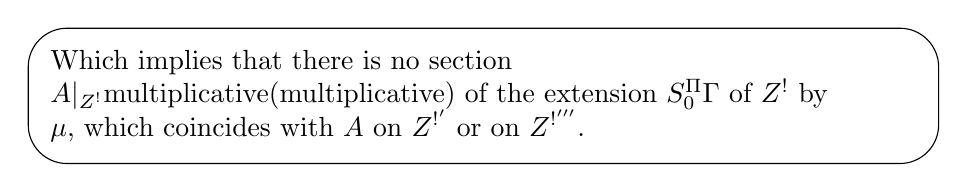
\begin{tikzpicture}
\node[draw,rounded corners=14pt,inner sep=8pt,text width=11cm,align=left]
{Which \unsure{implies} that there is no section
\deleted{$\unsure{A|_{Z^!}}$\unsure{multiplicative}}\inserted{(multiplicative)}
of the extension $S_0^{\Pi}\Gamma$ of $Z^!$ by $\mu$, which coincides
with $A$ on $Z^{!'}$ or on $Z^{!'''}$.};
\end{tikzpicture}}}

We then have this:

a) $S_0^{\Pi_0}\Gamma^{!'},S_0^{\Pi_0}\Gamma^{!'''}$ are
\uline{not} \uline{normal} in $S_0^{\Pi}\Gamma^!$.

b) $S_0^{\Pi_0}\Gamma^{!0}$ is normal in
$S_0^{\Pi}\Gamma^!$, so that the extension
$S_0^{\Pi}\Gamma^!$ of $Z^!\simeq M^![0]$ by $\mu$
is canonically isomorphic to the inverse image of an
\unsure{extension|category} \inserted{central} and finite
$S_0^{\Pi}\Gamma^!/(S_0^{\Pi_0}\Gamma^{!0})$
of $Z^!/Z^{!0}\simeq\mu\times\mu$ by $\mu$.

\mspage{599}

\scanpage{601}
\mspage{604}

Let us examine this central extension
\[
(84)\qquad
\diagram{\begin{tikzcd}[ampersand replacement=\&,column sep=large,row sep=small]
1\arrow[r]\&\mu\arrow[r]\&
\mathcal E\arrow[r,"{(\varepsilon_3,\varepsilon_2)}"]
\arrow[d,phantom,"{\rotatebox{90}{$\simeq$}}" description]\&
\mu\times\mu\arrow[r]\&1\\
\&\&S_0^\Pi\Gamma_{\rho,\sigma}/S_0^{\Pi_0}\Gamma^0_{\rho,\sigma}\&\&
\end{tikzcd}}
\]
fitting into the diagram of extensions,
\[
(85)\qquad
\diagram{\begin{tikzcd}[ampersand replacement=\&,column sep=large,row sep=large]
1\arrow[r,dash]\&\mu\arrow[r]\&
\mathcal E\arrow[r,dash]\&\mu\times\mu\arrow[r,dash]\&1\\
1\arrow[r,dash]\&\mu\arrow[r]\arrow[u,"1"']\arrow[d,hook]\&
S_0^\Pi\Gamma^!_{\rho,\sigma}\arrow[r]\arrow[u]\arrow[d,hook]\&
Z^!_{\rho,\sigma}\arrow[u,"{(\varepsilon_3,\varepsilon_2)}"']
\arrow[d,leftrightarrow,"1"]\arrow[r,phantom,"{\simeq M[0]}" description]\&\vphantom{1}\\
1\arrow[r]\&L_\rho\times L_\sigma\arrow[r]\&
S_0\Gamma^!_{\rho,\sigma}\arrow[r]\&Z^!_{\rho,\sigma}\arrow[r]\&1
\end{tikzcd}}
\]

The interest of (84) is that it allows one to recover the extension
$S_0\Gamma_{\rho,\sigma}$ of $Z^!_{\rho,\sigma}$ by
$L_\rho\times L_\sigma$, by the \unsure{covariant}-\unsure{contravariant}
\unsure{law} in the functor
``extensions'', from
\[
(86)\qquad
\diagram{\begin{tikzcd}[ampersand replacement=\&,column sep=large,row sep=small]
Z^!_{\rho,\sigma}\arrow[r,"{(\varepsilon_3,\varepsilon_2)}"]\&
\mu\times\mu
\end{tikzcd}},\qquad
\begin{gathered}
\diagram{\begin{tikzcd}[ampersand replacement=\&,column sep=large,row sep=small]
\mu\arrow[r,hook]\&L_\rho\times L_\sigma\\
-1\arrow[r,mapsto]\&(\rho^3,\sigma^2)
\end{tikzcd}}\\
\text{(``diagonal homomorphism'')}
\end{gathered},
\]
as well as the subextension $S_0^\Pi\Gamma^!_{\rho,\sigma}$ of
the latter (of $Z^!_{\rho,\sigma}$ by $\mu$).

Let us first study the order of the elements of $\mathcal E$ --- they are
obviously divisors of $4$, are they all of order $2$ (or $1$)? Let
\[
\underline{\unsure{\bar u|u}}=
\left(
\underset{\inserted{\substack{\rotatebox{90}{$\in$}\\Z}}}{u},
\underset{\inserted{\substack{\rotatebox{90}{$\in$}\\N_\rho^*}}}{a},
\underset{\inserted{\substack{\rotatebox{90}{$\in$}\\N_\sigma^*}}}{b}
\right)\in S_0^\Pi\Gamma^!
\qquad\text{i.e.}\quad
\left\{\begin{aligned}
u&\equiv b\quad(\widehat\Pi_0)\\
u&\equiv\varepsilon_3[\sigma]a\quad(\widehat\Pi)
\end{aligned}\right.
\qquad(87)
\]
\margin{\uline{N.B.} To \unsure{prevent|introduce} confusions,
\unsure{I write} $\varepsilon_3[\sigma],\varepsilon_3[\tau']$
in preference \unsure{to|of} $\varepsilon_3(\sigma),\varepsilon_3(\tau')$
for $\sigma^{\unsure{\nu_3}},\tau'^{\unsure{\nu_3}}$.}

I \deleted{\unsure{want}} want to examine whether
$\underline{u}^{2}\in S_0^{\Pi_0}\Gamma^{!0}$.
Obviously
\[
\underline{u}=(u^2,a^2,b^2)\in S_0^\Pi\Gamma^{!0}
\]

\mspage{600}

\scanpage{602}

it remains to see whether $\underline u^{2}\in S_0^{\Pi_0}\Gamma^{!}$, i.e. whether we have
\deleted{\unsure{not}} only
$\unsure{u^{2}}\equiv b^{2}\ (\Pi_0)$ and
$\deleted{\unsure{a^{2}}}\unsure{u^{2}}\equiv a^{2}\ (\widehat\Pi)$
--- which is clear and simply expresses
$\underline u^{2}\in S_0^{\Pi}\unsure{\Gamma|\Gamma^{!}}$ --- but even
\[
\tag{88}
\unsure{u^{2}}\equiv a^{2}\quad\bmod\ \uuline{\widehat\Pi_0}
\qquad (?)
\]

The relation
\[
u\equiv\varepsilon_3[\sigma].a\quad\bmod\Pi
\]
can also be written
\[
u\equiv\pm\varepsilon_3[\sigma].a\quad\bmod\Pi_0
\]
and implies
\[
u^2\equiv\varepsilon_3[\sigma]a\ \varepsilon_3[\sigma]a
\quad\bmod\Pi_0
\]
which we can write
\[
\tag{89}
\underset{\bmod\widehat\Pi_0}{u^2\equiv
\varepsilon_3\,\varepsilon_3[\sigma](a).a}
=\begin{cases}
a^2&\text{if }\varepsilon_3=1.\\
-\sigma(a).a&\text{if }\varepsilon_3=-1
\end{cases}
\]

Thus (88) is true if $\varepsilon_3=1$, whereas
for $\varepsilon_3=-1$, it is equivalent to
\[
\sigma(a)\equiv-a\qquad(\widehat\Pi_0)
\]
i.e.
\[
[\sigma,a]^{\cdot}=-1\quad\text{in }\unsure{\widetilde{\mathcal G}|\widetilde{\mathcal C}}/\Pi_0
\]
i.e.
\[
\underbrace{\varepsilon_2(a)}_{\inserted{\begin{gathered}\rotatebox{90}{$=$}\\\varepsilon_2(u)\end{gathered}}}=-1
\qquad\text{i.e. }\varepsilon_2(\unsure{u})\varepsilon_3(\unsure{u})=1.
\]

Thus we find:

\uline{Proposition} Let $x\in\mathcal E$ (cf. (84)). For
$x^2=1$ to hold, it is necessary and sufficient that we have
$\varepsilon_3(x)=1$ \uline{or} $\varepsilon_2(x)\varepsilon_3(x)=1$,
i.e. that
\deleted{$x$ \unsure{belong to the subgroup} $\mathcal E'$ \unsure{or}}
\inserted{we have}
\[
\tag{90}
x\in\mathcal E'\cup\mathcal E''',
\]

\mspage{601}

\scanpage{603}
\mspage{605}

where
\[
\tag{91}
\mathcal E'=\{\unsure{x|n}\in\mathcal E\mid\varepsilon_3(x)=1\},\qquad
\mathcal E'''=\{\unsure{x|n}\in\mathcal E\mid\varepsilon_2(x)\varepsilon_3(x)=1\}
\]

\uline{Corollary 1} $\mathcal E$ has exactly two elements
of order $4$, which are the two elements of $\mathcal E$
above the element $(-1,1)$ of $\mu\times\mu$.
These two elements are inverses of one
another, \unsure{these|and} are the two generators of
the only cyclic subgroup of order $4$ of $\mathcal E$,
which is none other than
\[
\tag{92}
\mathcal E''=\{\unsure{x|n}\in\mathcal E\mid\varepsilon_2(x)=1\}
\]

\uline{Corollary 2} The extension $\mathcal E$ is not split.

For being central, it \deleted{\unsure{itself}} would be isomorphic
to $(\mu\times\mu)\times\mu$, so its elements would have order
dividing $2$.

We can now regard
$\mathcal E$ as an extension of $\mathcal E/\mathcal E''\simeq\{\pm1\}=\mu$ by
$\mathcal E''\ (\simeq\mathbb Z/4\mathbb Z)$.
\deleted{But it} It would be necessary
first to make explicit the operation of $\mathcal E/\mathcal E''=\mu$
on $\unsure{\mathcal E'|\mathcal E''}$ --- the element \inserted{$-1$} of order $2$ of $\mu$
induces an involutive \unsure{automorphism} of \deleted{$\unsure{\mathbb Z/4\mathbb Z}$} $\mathcal E''$
\inserted{moreover in $\mathrm{Aut}(\unsure{\mathcal E'|\mathcal E''})\simeq
(\mathbb Z/4\mathbb Z)^*\simeq\{\pm1\}$, so
the automorphism in question}
\deleted{that \unsure{its}} is multiplication by a
sign $\varepsilon\ \pm1$, which has to be determined. We are going
to take \inserted{as representative of $-1\in\mathcal E/\mathcal E''$}
the element of $\mathcal E$ coming
\deleted{from}\inserted{from}
\[
\tag{92}
\deleted{\unsure{\tau,a',\tau}}\quad
\underline x=(u_0=\tau,\ a_0=\tau',\ b_0=\tau)
\in S_0^{\Pi_0}\Gamma^{!'''}\qquad(\text{cf.}(70))
\]
which we are going to have operate on the image of a
\[
\tag{93}
\underline u=(u,a,b)\in S_0^{\Pi}\Gamma^{!},\quad
\deleted{\unsure{\text{where}}}\ \text{with }\varepsilon_3(u)=-1,\ \varepsilon_2(u)=1
\]
\inserted{\[
\left(\begin{array}{ll}
u\equiv b\ \deleted{\unsure{\equiv a}}&\bmod\widehat\Pi_0\\
u\equiv\sigma a&\bmod\widehat\Pi
\end{array}\right)
\]}
(which is a generator of $\mathcal E''$).

\mspage{602}

\scanpage{604}

We shall thus have
\[
\underline x(\underline u)=(\tau(u),\tau'(a),\tau(b))\equiv
\deleted{\unsure{(u,\varepsilon a,\varepsilon b)|(\varepsilon u,\varepsilon a,\varepsilon b)}}
\underbrace{\inserted{(1,\varepsilon,\varepsilon)(u,a,b)}}_{\inserted{(u,\varepsilon a,\varepsilon b)}}
\]
modulo $S_0^{\Pi_0}\Gamma^{\unsure{!0|0}}$, with a sign
$\varepsilon\in\{\pm1\}$ to be determined. The congruence condition can be written
\[
(u\tau(u)^{-1},\ \varepsilon a\tau'(a)^{-1},\
\varepsilon b\unsure{\tau'(b)|\tau(b)}^{-1})\in S_0^{\Pi_0}\Gamma^{\unsure{!0|0}}
\]
that we are in $S_0^\Pi\Gamma^{!0}$ is obvious,
\deleted{\unsure{the choice}}
\deleted{\unsure{immaterial|independent}}
\inserted{\unsure{valid|valid}}
whatever the choice of the sign
$\varepsilon$, \deleted{\unsure{it is}}
\deleted{\unsure{it is|and}}\inserted{\unsure{it is}}
\unsure{the|the} \unsure{condition|conditions} of congruence
\deleted{which} \deleted{\unsure{are essential}}
\inserted{which \unsure{distinguishes|distinguish} $S_0^{\Pi_0}\Gamma^{!}$ from
$S_0^\Pi\Gamma^{!}$ which is}
essential, namely
\[
\tag{94}
u\tau(u)^{-1}\equiv\varepsilon\unsure{a}\tau'(\unsure{a})^{-1}
\qquad(\widehat\Pi_0)\qquad\text{i.e.}
\]
\deleted{\[
\unsure{u(\tau)\tau^{-1}\equiv\varepsilon a(\tau')\tau'^{-1}}
\]}

The difficulty with this approach comes
from the fact that the only elements of
$M$ that we know how to make explicit are those
coming from $\unsure{\widetilde{\mathcal G}|\widetilde{\mathcal C}}\simeq\mathrm{Gl}(2,\mathbb Z)$
itself; now
for these we have $\varepsilon_2(u)\varepsilon_3(u)=1$, whereas
the $u$-\inserted{here} \deleted{\unsure{test}} above must satisfy
$\varepsilon_2(u)=1$, $\varepsilon_3(u)=-1$ so
$\varepsilon_2(u)\varepsilon_3(u)=-1$.
We \unsure{can} on the other hand work in the
\deleted{\unsure{\text{group}} $\unsure{\widetilde{\mathcal G}|\widetilde{\mathcal C}}$}
\inserted{quotient} $\mathrm{Gl}(2,\widehat{\mathbb Z})$ of
\deleted{$\unsure{\widetilde{\mathcal G}|\widetilde{\mathcal C}}$} $M$, and
take in it
\[
\tag{95}
u=\begin{pmatrix}\mu&0\\0&1\end{pmatrix}
\quad\text{with}\quad
\mu\in\widehat{\mathbb Z}^{*},\quad
\begin{cases}
\mu\equiv-1&(3)\\
\mu\equiv1&(4)
\end{cases}
\]
\inserted{\[\text{i.e.}\quad\mu\equiv5\quad(12)\]}
whereas $\tau$ corresponds to the
matrix
\[
\tau=\begin{pmatrix}-1&0\\0&1\end{pmatrix}
\]

\margin{$\unsure{\wedge}$}
\mspage{603}

\scanpage{605}
\mspage{606}

we shall in any case have
\[
u\tau(u)^{-1}=1
\]
let, on the other hand, in $\mathrm{Gl}(2,\widehat{\mathbb Z})$
\[
\tag{96}
\left\{\begin{array}{lll}
a=\tau'a_0&a_0=c\rho+d&c^2+cd+d^2\in\widehat{\mathbb Z}^{*}\\[3pt]
&\tau'=\begin{pmatrix}0&1\\1&0\end{pmatrix},&
\rho=\begin{pmatrix}0&1\\-1&1\end{pmatrix}
\end{array}\right.
\]
\unsure{thus|whence}
\[
\tag{97}
a=\begin{pmatrix}0&1\\1&0\end{pmatrix}
\begin{pmatrix}d&c\\-c&c+d\end{pmatrix}
=\begin{pmatrix}-c&c+d\\d&c\end{pmatrix}
\]
and
\[
\tag{98}
\mu=-(c^2+cd+d^2)
\]

\margin{\unsure{a little brief}... cf. below...}

We \deleted{\unsure{are going to}} work with the closed \inserted{sub-}group
$\widehat\Pi_0$ in $\mathrm{Sl}(2,\widehat{\mathbb Z})$ generated by
\[
\begin{gathered}
-\ell_0\underset{\unsure{,}}{\unsure{=}}\unsure{-}\begin{pmatrix}
1&-2\\\deleted{\unsure{-2|2}}0&1
\end{pmatrix},\qquad
-\ell_1=-\begin{pmatrix}1&0\\2&1\end{pmatrix},\qquad
-\ell_\infty=-\begin{pmatrix}3&-2\\2&-1\end{pmatrix}
\end{gathered}
\]
and in the quotient group of
$\mathrm{Gl}(2,\widehat{\mathbb Z})$ by $\widehat\Pi_0$, which is
\deleted{\unsure{the}} the extension of
$\widehat{\mathbb Z}^{*}$ by
\[
\mathrm{Sl}(2,\widehat{\mathbb Z})/\widehat\Pi_0
\simeq\mathrm{Sl}(2,\mathbb Z)/\Pi_0
\simeq\left\{(\rho,\sigma)\ \left|\begin{array}{l}
\rho^6=\sigma^4=1\\
\rho^3=\sigma^2\\
\sigma(\rho)=\rho^{-1}
\end{array}\right.\right\},
\]
\deleted{\unsure{with}} and \unsure{this|in} a $\frac12$ direct product thanks to
\[
T_0=\left\{\begin{pmatrix}
\deleted{\unsure{\xi}}\unsure{\zeta|\xi}&0\\0&1
\end{pmatrix}\ \middle|\ \unsure{\zeta|\xi}\in\widehat{\mathbb Z}^{*}\right\}
\overset{\det}{\simeq}\widehat{\mathbb Z}^{*},
\]
operating through $\varepsilon_2(\unsure{\zeta|\xi})$
--- cf. pages $593'$, $594$ --- formulas (34)(35)(35 bis) ].
We \inserted{must} suppose
\[
\tag{99}
\sigma a\equiv u\qquad(\widehat\Pi_{\unsure{0}})
\qquad\text{where }\sigma=\begin{pmatrix}0&-1\\1&0\end{pmatrix}
\]
thus
\[
\tag{100}
\sigma a=\begin{pmatrix}-d&-c\\-c&c+d\end{pmatrix}
\]

\mspage{604}
